\section{Method}
\label{sec:method}


\begin{figure*}[t]
\centering
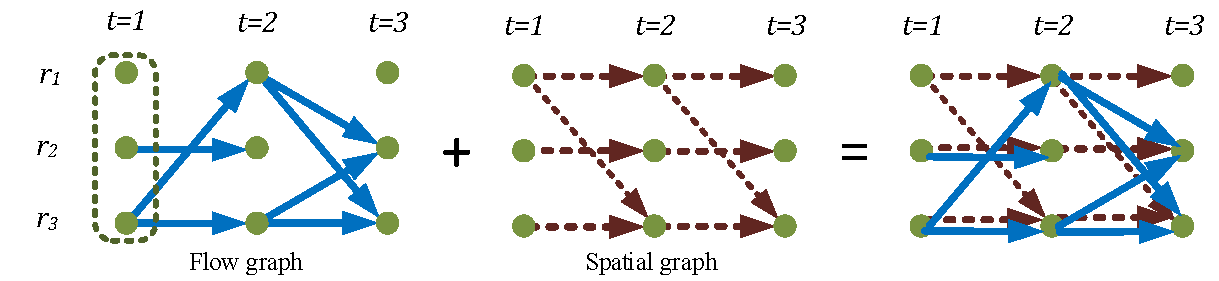
\includegraphics[width=1\linewidth]{fig/layered-graph-embedding.pdf}
\caption{The layered structure of a flow graph (left), a spatial graph (middle), and the combined graph (right). Each row $r_k$ is the region.  Each column $t$ is the timestamp, and all vertices within at the same timestamp (the dotted rectangle) form one \emph{layer} of the graph. Each vertex $v_i^t$ is a \emph{time-enhanced vertex} refers to region $r_i$ at time $t$. On the left, the solid blue edge refers to the taxi flow, and edge weight is number of taxi trips. In the middle, the dotted red edge refers to the spatial adjacency, and the edge weight is inversely correlated with the distance between region centroids. From the flow graph, vertices $v_1^2$ and $v_3^2$ have similar embeddings because they have similar in-flow from $v_3^1$ and similar out-flow to $v_2^3$ and $v_3^3$. However, with flow graph alone, we are not able to learn the embeddings for $v_1^1$ and $v_1^3$, due to lack of traffic flow. The spatial graph provides spatial information, which makes it possible to learn an embeddings for $v_1^1$ and $v_1^3$.}
\label{fig:layered-graph}
\end{figure*}




In this section, we give the design motivations and formal definitions of the flow graph and spatial graph. Following the graph definitions, we describe the embedding learning objective. At last, we present the optimization techniques to learn the embedding.



\subsection{Flow Graph}
\label{sec:method:transition-graph}

The same region at different time may carry different functions. Take the downtown area as example, which has mixed point-of-interests distribution. In the morning, people go to downtown mostly for work. Therefore, in the morning the downtown area acts as a professional area. However, at night there are also a significant amount of people travel to downtown for food and drink, and the downtown acts as an entertainment area.

The aforementioned example motivates us to learn different embeddings for the same region at different times. Follow this intuition, we design the flow graph $G_f$ as a layered graph, shown on the left of Figure~\ref{fig:layered-graph}, and formally defined as follows.


\begin{definition}[Flow graph]
The \emph{flow graph} is a layered graph defined as $G_f = (\V, E_f)$. The vertices $\V = \{ v_i^t \}$ is the set of time-enhanced vertex. The vertices with the same timestamp are grouped into one \emph{layer}, and there are $T$ layers in total.  The edge set $E_f$ only contains one type of edges $\{ e_{ij}^t \}$, where $e_{ij}^t$ connects vertices $v_i^t$ and $v_j^{t+1}$ from two consecutive layers. The edge weight $f_{ij}^t$ is the volume of mobility flow.
\end{definition}


The flow graph models the mobility pattern of crowd in the city. More specifically, we can sample a lot of paths from the flow graph to represent human trajectories. Each path consists of a sequence of regions, whose timestamps are monotonically increasing with a fixed step of 1. The length of each path is bounded by the number of timestamps in the graph. And each path semantically refers to one trajectory of a individual. For example, one possible path is $\langle \text{home, 8:00 am} \rangle \rightarrow \langle \text{office, 9:00 am} \rangle \rightarrow \cdots \rightarrow \langle \text{office, 6:00 pm} \rangle \rightarrow \langle \text{bar, 7:00 pm} \rangle $.


However, there are three issues with a path sampled from the flow graph. First, the flow graph does not deal with the fact that people travel to a region and stay there. For example, in the left-most graph in Figure~\ref{fig:layered-graph}, the edge between $v_1^1$ (node of region $r_1$ at time $t=1$) and $v_1^2$ (node of region $r_1$ at time $t=2$) is missing, which means there is no trip observed transiting within the same region, but there could be people staying in that region. Second, the flow graph suffers data sparsity issue. If there is no traffic flow going in/out some region during a time slot, then it is impossible to learn the embedding of this region at that time. Third, the flow graph cannot recognize the same or nearby region across different time slots. More specifically, the flow graph treats all $K \cdot T$ vertices as independent regions. However, it is very likely that the same region in different time slots are strongly correlated. Recall the residential area example, where the large volume of in-going flow at night is caused by the large volume of out-going flow in the morning.







\subsection{Spatial graph}



To address the issues with the flow graph, we propose a spatial graph, which is defined as:
\begin{definition}[Spatial graph]
\label{def:g_s}
The \emph{spatial graph} is a layered graph as well, denoted as $G_s = (\V, E_s)$. The  vertices set $\V$ is exactly the same as that of flow graph. The edge set $E_s$ also only contains edges connecting two vertices from consecutive layers. The edge weight $g_{ij}^t$ represent the spatial similarity of two regions, which is inversely correlated with distance.
\end{definition}

The spatial graph share the same structure and exactly the same vertices with the flow graph. The only difference is that the edges in spatial graph are constructed differently. The basic assumption behind the spatial graph is that human mobility are bounded by space. When there is no transition observed, the probability that people appeared at a different region is inversely correlated to the distance they need to travel. Therefore, two regions that are close in space should have stronger correlation in their embeddings. In spatial graph, the edges $e_{ij}$ refers to the spatial similarity between regions $r_i$ and $r_j$. The edge weight $g_{ij}$ is inversely correlated with the distance, formally defined with exponential decay function~\cite{nekola1999distance} as follows
\begin{equation}
g_{ij} = \exp ( - C \cdot d_{ij} ),
\end{equation}
where $d_{ij}$ is the spatial distance between the centroids of two regions. We should notice that the spatial graph is static over time, therefore, all edges between any two consecutive layers are actually the same. $C$ is a parameter controls the exponential decay rate of the distance. Larger $C$ means faster decay, which makes regions far away has little correlation with current region.





The design of spatial graph, shown in the middle of Figure~\ref{fig:layered-graph}, naturally incorporates the spatial adjacency. This spatial adjacency could be regarded as a transition cost, which helps us to estimate the stay probability. Even more, the spatial adjacency enables the embedding learning for regions without any taxi flow, which solves the sparsity issue. Lastly, the spatial adjacency identifies the same region across different timestamps, because the edge weight between a pair of time-enhanced vertices on the same region is always the maximum edge weight. 




\subsection{Heterogeneous Graph Property}

Combine the flow graph and spatial graph together, we get a heterogeneous graph that represents the crowd mobility pattern on the right of Figure~\ref{fig:layered-graph}. In this heterogeneous graph, one path convey more information about crowd mobility pattern than one path from the flow graph. Now it is possible for a path to capture both transition and stay, such as $\langle \text{home, 8:00 am} \rangle \rightarrow \langle \text{office, 9:00 am} \rangle \xrightarrow{\text{\bf stay}} \langle \text{\bf office, 10:00am} \rangle \rightarrow \cdots \rightarrow \langle \text{office, 6:00 pm} \rangle \rightarrow \langle \text{bar, 7:00 pm} \rangle $.

This heterogeneous graph has two properties that fit the requirement of our problem. (1) The graph is still a temporal graph, which enables us to learn a dynamic embedding for each region. (2) In the heterogeneous graph, the multi-hop temporal dependency is captured within each path. The multi-hop temporal dependency is important to differentiate region functions. For example, at 6:00 pm we observe same amount of flow going into region A and B, which makes it difficult to differentiate the function of A and B. But if we know that in the morning, there is a large amount of flow going out of A, while almost no flow going out of B, then A is more likely to be a residential area, whereas B is more likely to be an after-work entertainment region.




\subsection{Embedding Learning Objective}

In order to capture two properties mentioned above, we propose to use the embedding technique to learn the representation of each region. The reason is that graph embedding explicitly captures the multi-hop dependency. Meanwhile, the baseline method for graph representation learning, such as directly using the in/out flow as vector representation or matrix factorization,  is not able to capture the multi-hop correlation.

\subsubsection{On Single Graph}

The embedding learning process on the flow graph and the spatial graph are exactly the same, due to the fact that both graphs have similar structure. Without loss of generality, we take the flow graph as example to explain the learning process.


First we define a path as $P_i = v_{i_1} v_{i_2} \cdots v_{i_m}$, whose starting and ending vertices are $v_{i_1}$ and $v_{i_m}$ respectively. We omit the time superscript, because the time slots for the vertices of path $P$ must be monotonically increasing with fixed step size 1. And we denote the relation that a path contains a vertex $v_i^t$ as $v_i^t \in P$. With the definition of path, we further define the set of paths containing $v_i^t$ as $\mathcal{P}(v_i^t) = \{ P_i | v_i^t \in P_i \}$. The context of one vertex $v_i^t$, which refers to all the other vertices that are multi-hop neighbors of $v_i^t$, is defined as $C(v_i^t) = \{ v_c |  \exists P_i \in \mathcal{P}(v_i^t),  v_c \in P_i \} \diagdown \{v_i^t\} $.


We adopt the skip-gram model~\cite{mikolov2013efficient} to learn the embedding $\uv_i^t$ for each node $v_i^t$.  Formally, we estimate
\begin{equation}
\label{eq:cp_real}
p_f(v_c | v_i^t) = \frac{\exp({\uv_i^t}^T \uv_c)}{\sum_{v_{i^*} \in C(v_i^t)} \exp({\uv_i^t}^T \uv_{i^*})},
\end{equation}
where $v_c$ is one vertex in $v_i^t$'s context $C(v_i^t)$, $\uv_c$ and $\uv_i^t$ are the embeddings of $v_c$ and $v_i^t$ respectively.


The empirical conditional probability $\hat{p_f}(v_c | v_i^t)$ is estimated by the volume of mobility flow in the flow graph. More specifically, if $v_c$ is within the context of $v_i^t$, there must be at least one path from $v_c$ to $v_i^t$ or a path from $v_i^t$ to $v_c$. Without loss of generality, we assume one of the path is from $v_i^t$ to $v_c$ with $m$ vertices, denoted as $P_i$, where $v_{i_1} = v_i^t$ and $v_{i_m} = v_c$. First we estimate the transition probability of two adjacent vertices. Then the empirical probability $\hat{p_f}(v_c | v_i^t)$ is estimated from this transition probability.

The transition probability between two directly connected vertices  $v_{i_k}^t$ and $v_{i_{k+1}}^{t+1}$ is given by
\begin{equation}
\label{eq:pair-prob}
p(v_{i_{k+1}}^{t+1} | v_{i_k}^t) = \frac{f_{i_k i_{k+1}}^t} {\sum_{v_{j^*}\in N(v_i^t)} f_{i_k j^*}^t},
\end{equation}
where $N(v_i^t)$ refers to the direct next-hop neighbors of vertex $v_i^t$, and $f_{i_k i_{k+1}}^t$ refers to the weight of edge $e_{i_k i_{k+1}}^t$ in the flow graph. Therefore, the transition probability from $v_{i_1}$ to $v_{i_m}$ through $P_i$ is
\begin{multline}
\label{eq:transition}
p(P |v_{i_1}) = p(v_{i_m}, v_{i_{m-1}}, \cdots, v_{i_2} | v_{i_1}) \\
= \prod_{k}^m p(v_{i_k} | v_{i_{k-1}}, v_{i_{k-2}}, \cdots, v_{i_1})
\end{multline}
Due to the Markov property, Equation~(\ref{eq:transition}) becomes
\begin{equation}
p(P | v_{i_1}) = \prod_k^m p( v_{i_k} | v_{i_{k-1}}),
\end{equation}
The empirical conditional probability $\hat{p_f}(v_c | v_i^t)$ is
\begin{equation}
\label{eq:cp_emp}
\hat{p_f}(v_c|v_i^t) = \sum_{P_i \in \mathbb{P}} p(P_i | v_i^t),
\end{equation}
where $\mathbb{P}$ is the set of all paths starting at $v_i^t$ and ending at $v_c$.
Finally, we can learn the embedding by minimizing the difference between two distributions $p_f(v_c|v_i^t)$ and $\hat{p_f}(v_c | v_i^t)$. The objective is
\begin{equation}
\label{eq:obj_gt}
O_f = D(p_f(\cdot|\cdot), \hat{p_f}(\cdot|\cdot)),
\end{equation}
where $D$ is the distance function for two distributions, and one commonly used function could be the KL divergence. 



The embedding learning objective of spatial graph is similar to the flow graph. We minimize the difference between the embedding distribution and empirical distribution, which is
\begin{equation}
\label{eq:obj_gs}
O_s = D(p_s(\cdot|\cdot), \hat{p_s}(\cdot|\cdot)).
\end{equation}


\subsubsection{On Heterogeneous Graph}

In order to learn our embedding on two graphs simultaneously, we combine Equation~(\ref{eq:obj_gt}) and Equation~(\ref{eq:obj_gs}), and the joint learning objective is
\begin{equation}
O = O_f + O_s = D(p_f(\cdot|\cdot), \hat{p_f}(\cdot|\cdot)) + D(p_s(\cdot|\cdot), \hat{p_s}(\cdot|\cdot)).
\end{equation}



\subsection{Embedding Learning Optimization}


\subsubsection{On Single Graph}
\label{sec:sample}

Directly optimizing the objective in Equation~(\ref{eq:obj_gt}) and Equation~(\ref{eq:obj_gs}) is computationally expensive, due to two reasons. 
\begin{enumerate}
\item To calculate the conditional probability $p_f(\cdot | v_i^t)$ in Equation~(\ref{eq:cp_real}), for each $v_i^t$ it requires the summation over the entire set of vertices. Therefore, the overall complexity is $O(K^2\cdot T^2)$, where $K \cdot T$ is number of vertices.
\item To estimate the empirical conditional probability $\hat{p_f} (v_c | v_i^t)$ in Equation~(\ref{eq:cp_emp}), for every pair of vertices we have to sum over all paths $P_i$ among them, which is exponential to the number of vertices in one layer.
\end{enumerate}

To address the first problem, we adopt the negative sampling approach proposed in \cite{mikolov2013distributed}, which samples multiple negative pairs from a noise distribution to estimate one true pair. The objective is given by
\begin{equation}
\label{eq:cp_real_ns}
\log \sigma ( {\uv_i^t}^T \uv_c) + \sum_q^s \mathbb{E}_{v_q \sim P_n(v_i^t)} \left[ \log \sigma(- \uv_q^T \uv_c) \right],
\end{equation}
where $\sigma (x) = \frac{1}{1+\exp(-x)}$ is the sigmoid function, $P_n(v_i^t)$ is the noise distribution, and $s$ is the number of negative samples. The Equation~(\ref{eq:cp_real_ns}) is used to replace every $\log p(v_c | v_i^t) $ term during the skip-gram optimization.


\begin{figure}[t]
\centering
\begin{tikzpicture}[scale=0.85]
\draw (0,0) -- (1,1.6);
\draw (0,0) -- (1,-1.6);
\node [above left] at (0.5, 0.8) {$p_b = 0.2$};
\node [below left] at (0.5,-0.8) {$p_c = 0.8$};
\draw [fill=red, red, thick] (0,0) circle [radius=0.1];
\node [above left] at (0,0) {A};
\draw [fill=red, red, thick] (1,1.6) circle [radius=0.1];
\node [above right] at (1,1.6) {B};
\draw [fill=red, red, thick] (1,-1.6) circle [radius=0.1];
\node [below right] at (1,-1.6) {C};

\node  [below right] at (1.5, 2.1) {
\begin{tabular}{|c|c|c|c|}
\hline
Vertex & Index & Probability $p_i$ & Alias $K_i$ \\
\hline
B & 0 & 0.4 & C \\
\hline
C & 1 & 1.0 & - \\
\hline
\end{tabular}};

\node [below right] at (1.5, 0.6) {
\pbox[t]{\linewidth}{\em \textbf{Constant time sampling process}: \\
1. Draw uniform random number $x\in[0,1)$. \\
2. Identify the index of row $i = \lfloor n x \rfloor$. \\
3. If $x > p_i$, return $K_i$. Otherwise, return $i$. \\
Example 1: $x=0.45$, $i = 0$. Since $x > p_0$, return C.\\
Example 2: $x=0.35$, $i=0$. Since $x < p_0$, return B. }};
\end{tikzpicture}
\caption{The alias method explanation. On the left, we want to draw the next vertices of A. The probability table and alias table are created on the top right. The bottom right shows the constant time sampling process from the alias method.}
\label{fig:alias-method}
\end{figure}


To address the second problem, we use the graph sampling method to estimate the empirical probability $\hat{p}(v_c| v_i^t)$. More specifically, we generate $m$ paths from the graph via random walk. Due to the special structure of our layered graph, the time index of the sequence must be monotonically increasing with fixed step size 1. Given that $m$ is large enough, we could use the co-occur frequency count from those random walks to estimate $\hat{p}(v_c| v_i^t)$ with sufficient accuracy. 

The random walk boils down to next-vertex sampling according to the edge weights. Since the random walk is conducted on a weighted graph, at each vertex, we sample the next vertex according to the out-degree distribution, which could be expensive. The straightforward method is to convert each weighted edge into an interval within the range of $[0, w_{sum})$, where the $w_{sum}$ is the sum of out degree at current vertex. The sampling process is that first generate a uniform random number $x \in [0, w_{sum})$, and then find the interval that $x$ maps into. Therefore, this next-vertex sampling method takes $O(K)$ time, where $K$ is the number of vertices in one layer, which is also the upper bound of number of outgoing edges from current vertex. Since we are generating $m$ paths, we have to conduct $m \cdot T$ next-vertex sample process, where $T$ is the upper-bound of the path length. The overall complexity would be $O(m\cdot T\cdot K)$.

We further boost the next-vertex sampling process with alias method~\cite{walker1974new}. The advantage of alias method is that it is possible to repeatedly sample next edge with constant time, after preprocessing outgoing edges and save the information.  More specifically, the alias method creates two tables for the next edges as shown in Figure~(\ref{fig:alias-method}).  The alias method makes the path sampling significantly faster, because in  our path sampling process we repeatedly sample on each vertex. For each vertex, the initialization of alias tables take $O(K)$, where $K$ is the upper bound for the number of next vertex. Therefore, the overall initialization takes $O(K \cdot T \cdot K) = O(K^2 \cdot T)$, where $K \cdot T$ is the number of alias tables need to create. The overall sampling process takes $O(m \cdot T)$. Since $m \gg K$, it is safe to assume that $m > K^2$, and then the overall complexity is $O(K^2 \cdot T + m \cdot T) = O(m \cdot T)$. The experimental comparison of alias method with the simple method is described in Section~\ref{sec:runtime}.

%\todo{Probably mention the experiment to test different numbers of sampled random walks.}


\subsubsection{On Heterogeneous Graph}

The sampling-based method above can be easily applied on the heterogeneous graphs to learn the joint embedding. We conduct random walk on both graphs to generate path simultaneously. Then we feed all the paths to the skip-gram neural networks model to learn a joint embedding for each vertex.




\subsection{Discussion: Path Sampling}

Here we draw a connection between our graph sampling-based optimization technique and  word2vec~\cite{mikolov2013efficient} in language modeling method. The goal of word2vec is to build vector representations of words using probabilistic neural networks. This idea could be re-purposed to model the graph structure as well \cite{perozzi2014deepwalk}, due to the power law property in both the degree distribution in a graph and the word frequency distribution in natural language.

We regard the set of vertices in the graph as a special corpus, and each vertex is a word. The path sampled from the weighted graph via random walk can be thought of sentences. The multi-hop neighbors of a vertex in the path is similar to the word context. Therefore, estimating the neighboring vertices of a given vertex is analogy to the skip-gram language model~\cite{grovernode2vec}. 